\chapter{Implementation}\label{Implementation}

The first iteration of implementation was done through the use of the mathematical tool MATLAB; it consisted of 4 functions. The first received the data from the measuring box, the second decided an angle depending on the input from the user, the third selected a movement speed, and the last function wrote to the Teensy. Each function on its own was tested and was found to work separately. While implementing all the functions together in MATLAB a problem occurred with the communication between the computer, the measuring box and the Teensy. The problem may have been the buffer of the MATLAB which stores all data in a first in first out buffer (FIFO buffer). \\
After this setback, an implementation directly on the Teensy was done, while the only use of the computer was to debug and visualise the input from measuring box and the angles of the CrustCrawler. This was done through the use of a program called \textit{Telemetry}, that is made for telemetry on drones. This program plots the values it receives, by CSV (comma separated values). Below is a figure of the Telemetry GUI used for debugging the system.
\begin{figure}[H]
    \centering
    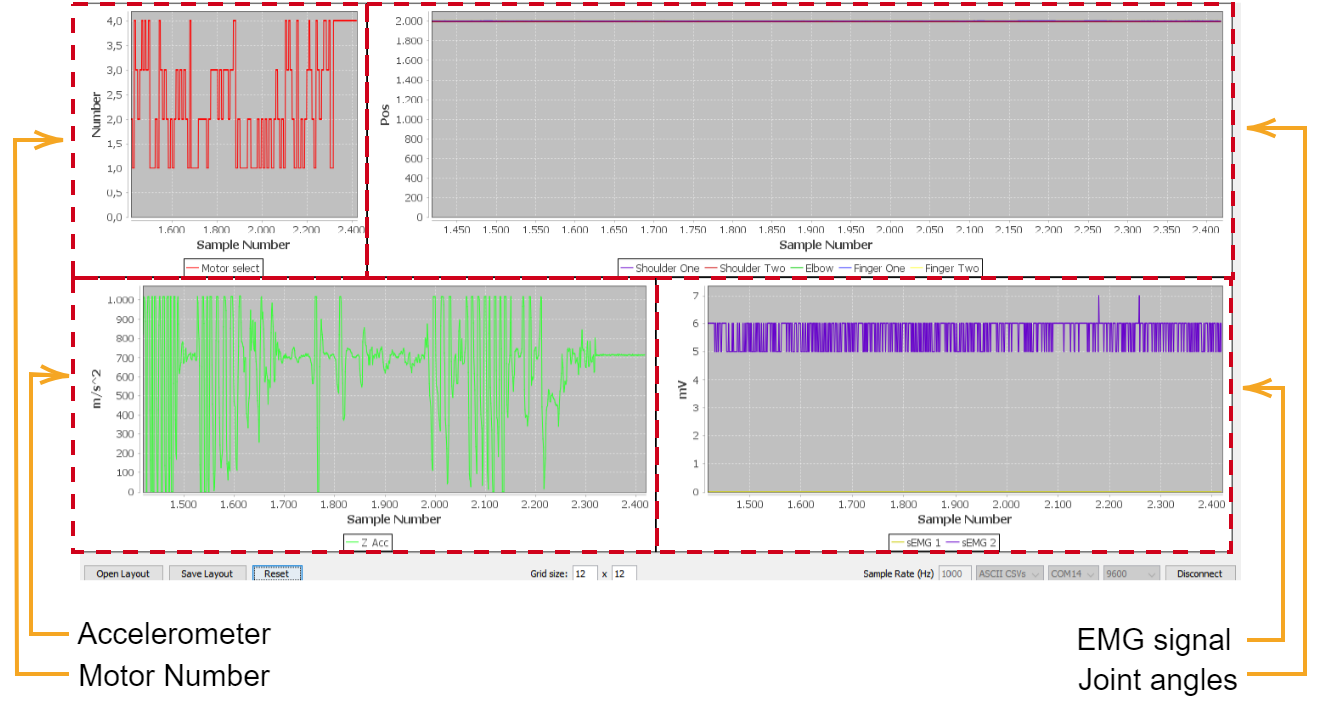
\includegraphics[width=0.79\textwidth]{Figures/Technical_figures/GUIla.png}
    \caption{GUI for debugging and setup}
    \label{fig:GUI}
\end{figure}
The use of Telemetry helped since the debugging and the setup of the prosthesis towards the user could be done visually instead of reading the outputs directly in the Arduino serial console.

Arduino is a program that can compile source code for the Arduino microcontroller , but there is add-on's to the Arduino program, that enables the Arduino compiler to compile and write to other microcontrollers such as the Teensy. The version of the Arduino compiler that is used in this project is the 1.8.6 there is a newer version, but that is not compatible with the Flexcan add-on that is used for communicating with the Teensy. In the next couple of sections these codes can be read.


\begin{figure}[H]
    \centering
    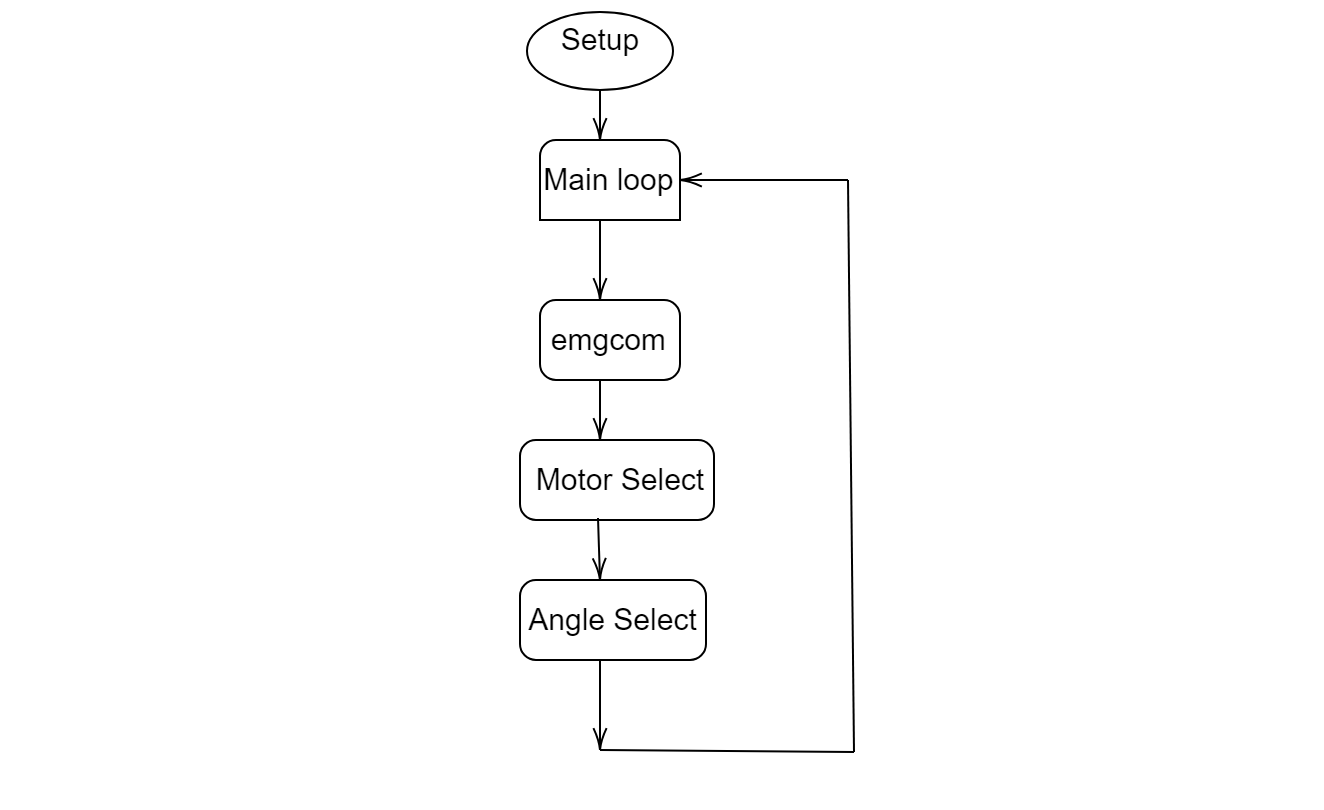
\includegraphics[width=\textwidth]{Figures/Technical_figures/diagen.png}
    \caption{The flowchart is a visual representation of how the main program is structured on the Teensy.}
    \label{fig:generalflowchart}
\end{figure}

\section{Software implementation}
In this section, there are descriptions of the different functions that are implemented on the Teensy. 
\subsection*{Measuring box}
\begin{figure}[H]
    \centering
    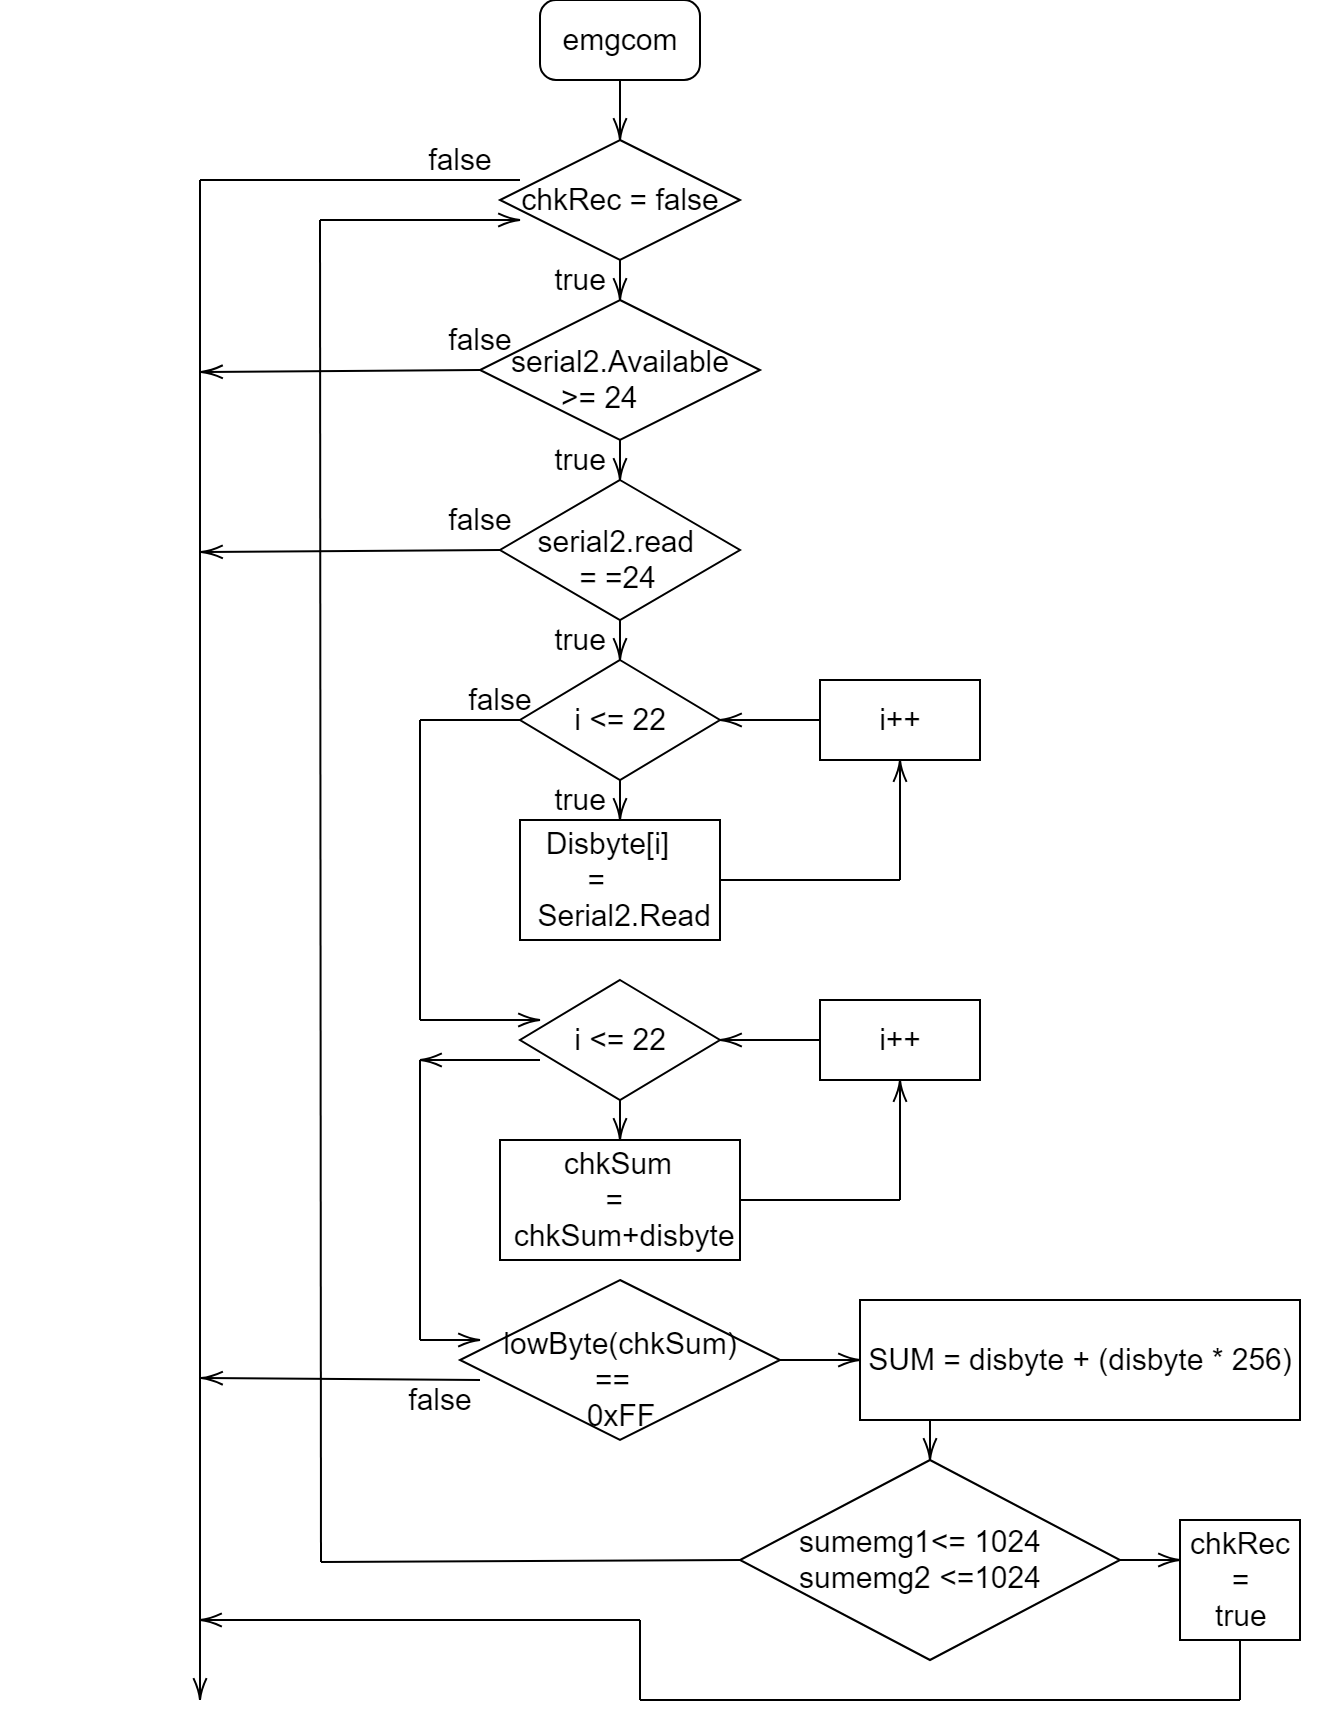
\includegraphics[width=\textwidth]{Figures/Technical_figures/emgcom.png}
    \caption{Flowchart of the "emgcom" code}
    \label{fig:emgcom}
\end{figure}
To get the data the measuring box provides there is a need to verify if data is correctly received.
The checksum Method is used to ensure the transmitted data has not been corrupted or disrupted.\\
The bytes excluding the Start delimiter, the Length bytes and the checksum will be referred to as the data-structure.\\
The Xbee checksum is calculated by adding all the bytes in the data structure, keeping only the 8 lowest bits in the result and subtracting it from 0xFF in hexadecimal(255 in Decimal)\cite{Calculat82:online}.
The sum of the data structure with the transmitted checksum added is 0xFF, if the transmission has not been altered \cite{XbeeManual:online}.

\subsubsection{Code explanation}
 \begin{figure}[H]
    \centering
\begin{lstlisting}[frame=single,language=Arduino] 
void emgCom(int &sumx, int &sumy, int &sumz, int &sumemg1, int &sumemg2 ) {
  byte disbyte[22];
  bool chkRec = false;
  while (chkRec == false) {
    if (Serial2.available() >= 24) {
      if (Serial2.read() == 126) {
        for (int i = 0; i <= 22; i++) {
          disbyte[i] = Serial2.read();
        }
        int chkSum = 0;
        for (int i = 2; i <= 22; i++) {
          chkSum = chkSum + disbyte[i];
        }
        if (lowByte(chkSum) == 0xFF) {
          sumz = disbyte[13] + (disbyte[12] * 256);
          sumy = disbyte[15] + (disbyte[14] * 256);
          sumx = disbyte[17] + (disbyte[16] * 256);
          sumemg1 = disbyte[19] + (disbyte[18] * 256);
          sumemg2 = disbyte[21] + (disbyte[20] * 256);
          if( sumemg1<=1024 && sumemg2 <=1024 ){
          chkRec = true;
          }
          else{}
        }
      }
    }
  }
  return;
}
\end{lstlisting}
    \caption{The source code for interpreting the data from the mearsuring box}
    \label{fig:EMG}
\end{figure}
 
\paragraph{Line 2-9}The array \textit{disbyte[22]} is made.
Then the Teensy search the data from the Xbee to look for the start delimiter which is 126 or 0x7E and stores the next 23 of bytes.
\paragraph{Line 10-13:}The int \textit{chkSum} is the sum of the data structure and the checksum byte. It is calculated by adding up the the bytes in the disbyte[22] array excluding the two length bytes from the Xbee.

\paragraph{Line 14-19}The \textit{chkSum} value is tested to ensure it has the value 0xFF. If this is true the sum of z acc., sum of y acc., sum of z acc., sum of emg1 and sum of emg2 are calculated to be used in another function.


\paragraph{Line 20} Due to the \textit{chkSum} in some instances can be 255 without being altered. One more check than the check sum is done through the \textit{if} statement where if the EMG signal is above 1024 then \textit{chkRec} will not be set true. This will keep the loop running till it has a correct packet.

\paragraph{Lowbyte and highbyte} Low byte is a term used when more than one byte is transmitted. The low byte refers to the byte that holds the least significant part of an integer. For any integer type the low byte stores the part of the integer consisting of the powers of to from $2^0$ to $2^7$ which mean that an integer with a value below 255 can be held in the low byte. The structure from the XBee is ordered from higbyte to lowbyte, meaning that the highbyte is the leftmost byte of a variable and the lowbyte is the rightmost byte. 

\paragraph{Test "Receiving data from measuring box"}
For this project to work a communication link between the Xbee and the Teensy needs to be established. The code was tested, but a flaw in the checksum meant that there was a need to isolate the problem, values that came through was above a certain threshold. After the implementation the if statement in \textit{line 20} in \ref{fig:EMG} the test of the communication was a success, it was able graph the output of the measuring box in the GUI.

\subsection*{MotorSwitch}\label{MotorSwitchCode}
\begin{figure}[H]
    \centering
    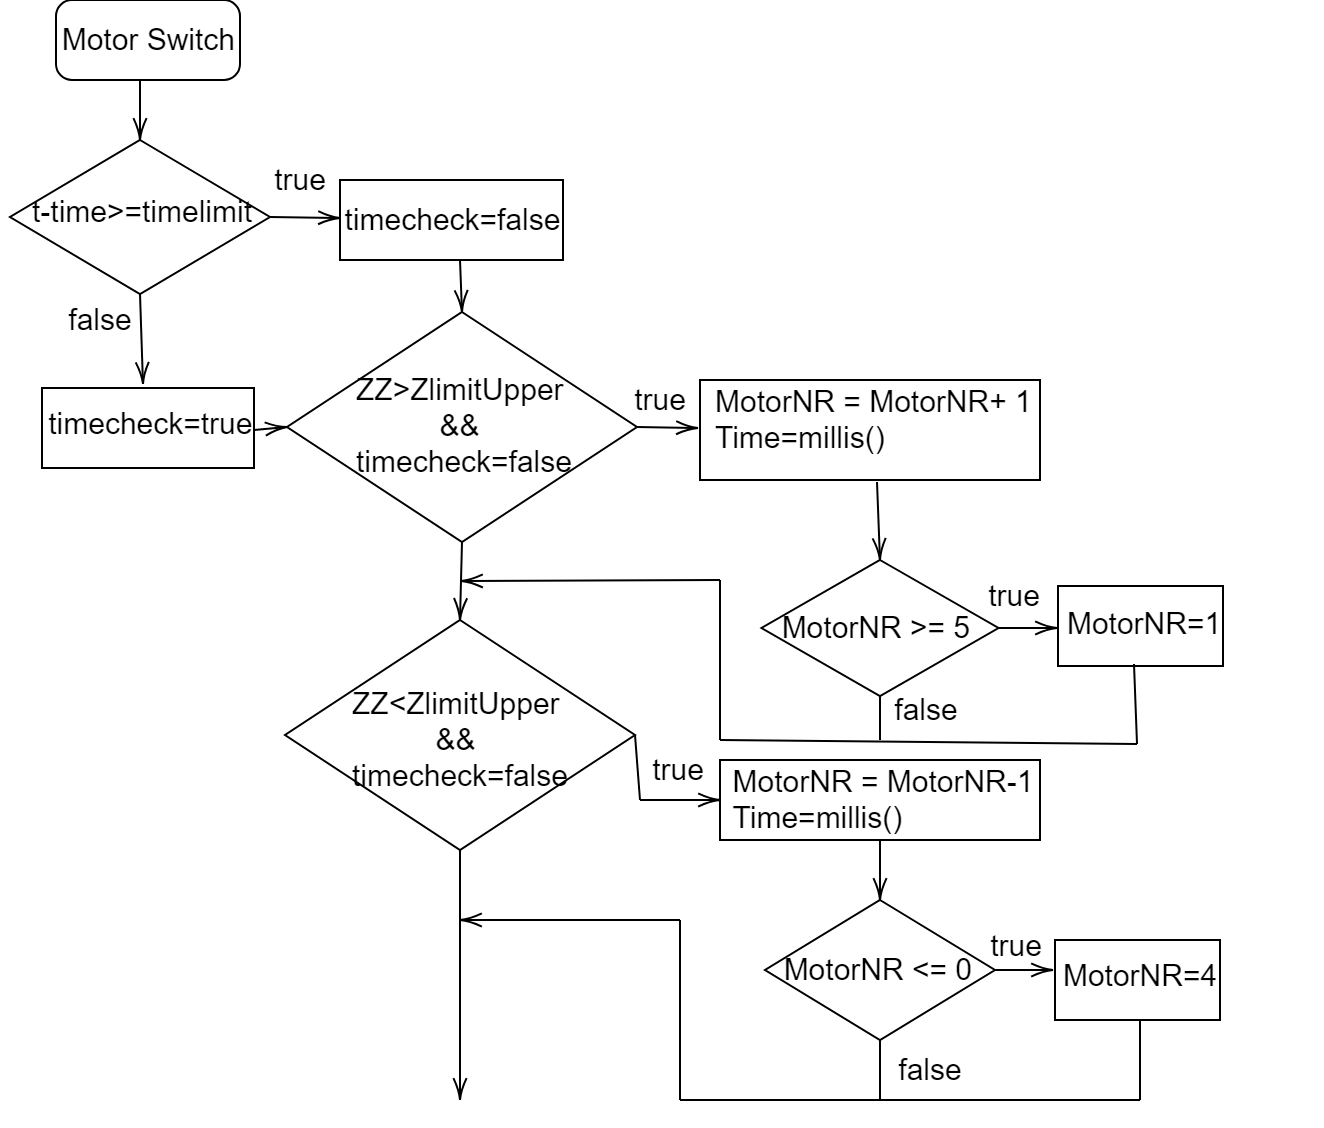
\includegraphics[width=\textwidth]{Figures/Technical_figures/motorselect.png}
    \caption{The flowchart of motor selection}
    \label{fig:motorsele}
\end{figure}
As shown below the code of switching the motors is presented. This code is a function implemented to control the signals of the accelerometer. This code makes use of the Z-axis, which is the axis it is meant to operate in when the user lifts the shoulder.\\

\begin{figure}[H]
    \centering
\begin{lstlisting}[frame=single,language=Arduino] 
void MotorSwitch(int &MotorNR, int DD,bool &timeCehk,unsigned long &Time){
    if (DD>800 && timeCehk==false){
        MotorNR = MotorNR + 1;
        timeCehk=true;
        Time = millis();
    }
     if (DD < 450 && timeCehk==false){
        MotorNR = MotorNR - 1;
        timeCehk=true;
        Time = millis();
    }
    if (millis() - Time >= 300){
      timeCehk=false;
    }
    if (MotorNR > 4){
        MotorNR = 1;
    }
     if (MotorNR < 1){
        MotorNR = 4;
    } 
    else{}
 }
\end{lstlisting}
    \caption{The source code for the motor switch}
    \label{fig:motorSel}
\end{figure}
\noindent
\paragraph{Line 1-5:} An initialisation is commenced with the variables it is wished to use.
\paragraph{Line 6-7} This if statement states that the t - time must be higher or equal to "Timelimit" to proceed in setting timecheck = false, so that the time taken to switch motors won't exceed a certain threshold, and to set timecheck = false so the other 2 if statements can be run.
\paragraph{Line 8-17}Two different if statements is produced. The first if-statement is only run if ZZ is over 850, and if timecheck is false. ZZ is the accelerometer's Z-axis acceleration. Timecheck is always false unless the if statement in line 6 is not true. The second if-statement states that if ZZ is below the lower limit of 500, it switches the motor in a negative direction.\\
MotorNR has a preset of 1, which means it is set to motor 1. When the different if statements is run the motor will switch respectively to the if statements.
\paragraph{Line 11 + 16}The last lines of code is simply to keep the motors from exceeding the number of motors available. E.g if MotorNR is lower than 0, then switch to motor 4 etc.
\paragraph{Test of "Motor selection"}
For the user to control each motor separately the function motor select was tested and was a success after adding in \textit{line 3, 4} the reason to this was that motor would change every time it looped the main loop if the accelerometer had a signal above or below the thresholds.  
\subsection*{Angleselect}
\begin{figure}[H]
    \centering
    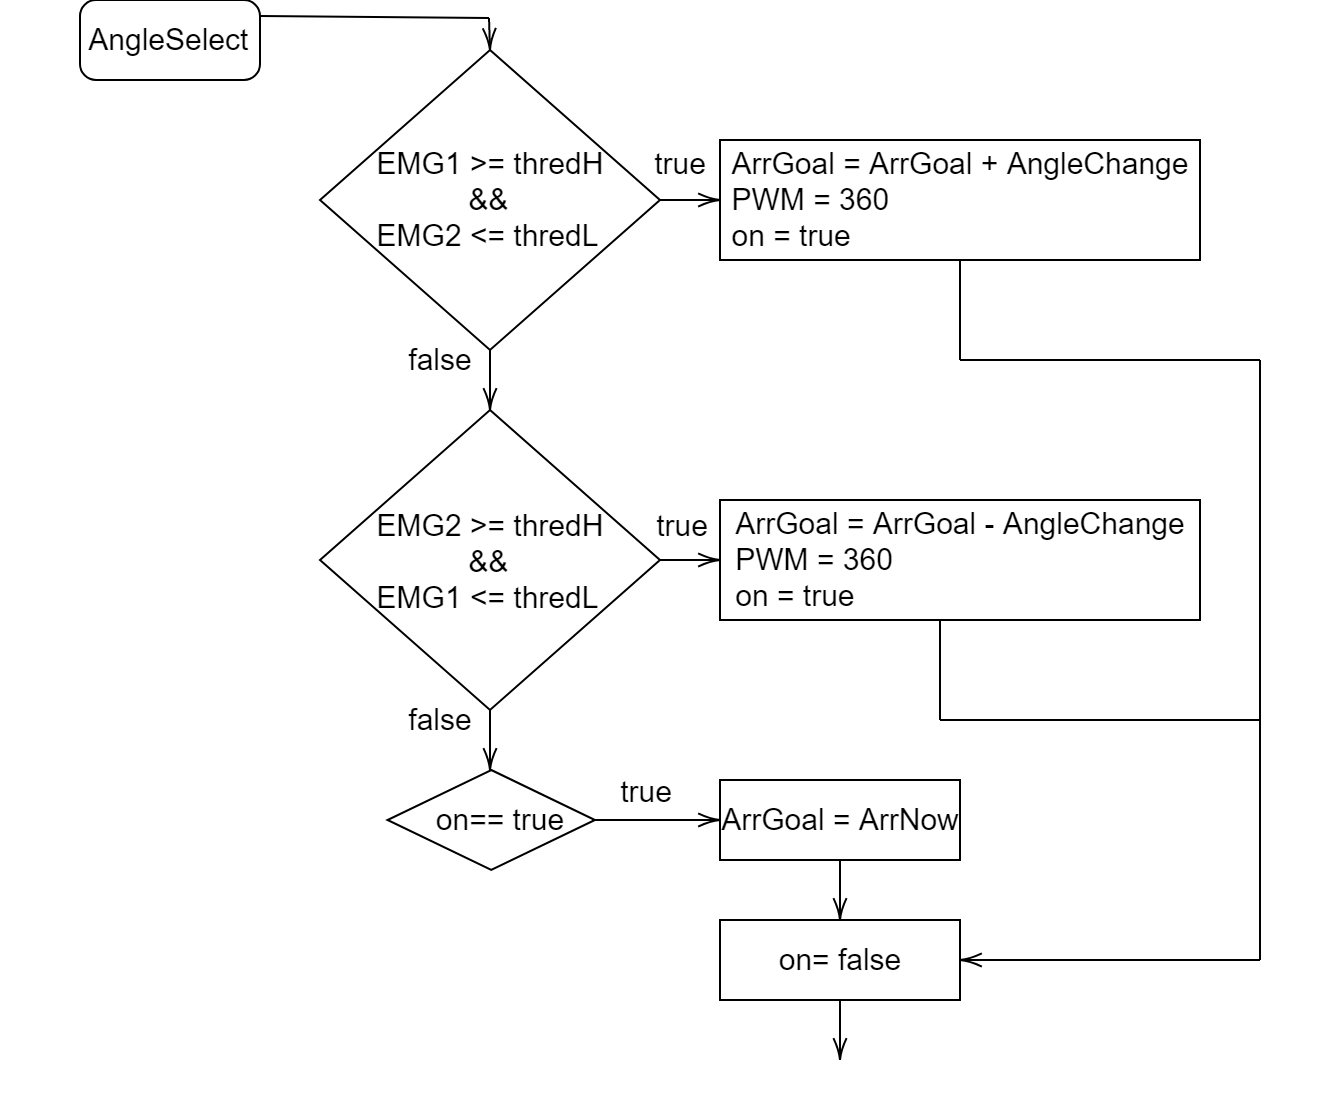
\includegraphics[width=\textwidth]{Figures/Technical_figures/angleselect.png}
    \caption{Flowchart of the angleselect code }
    \label{fig:angleSel}
\end{figure}
AngleSelect is a function that increases or decreases the angle of the manipulator. This makes the manipulator more manoeuvrable and easy to steer for the user.\\
\begin{figure}[H]
    \centering


\begin{lstlisting}[frame=single,language=Arduino]
void AngleSelect(int32_t &ArrNow, int &MotorNR, int &ArrGoal, int EMG_1, int EMG_2, int32_t &PWM, bool &on){
  int thredH = 50;
  int thredL = 50;
  int AngleChange = 10;
  if (MotorNR == 1){
    if (EMG_1 >= thredH && EMG_2 <= thredL){
      ArrGoal = ArrGoal + AngleChange;
      PWM = 360;
      on = true;
    }
    else if (EMG_2 >= thredH && EMG_1 <= thredL){
      ArrGoal = ArrGoal - AngleChange;
      PWM = 360;
      on = true;
    }
    else{
      if (on == true){
        ArrGoal = ArrNow;
      }
      on = false;
    }
  }
  else{
    if (EMG_1 >= thredH && EMG_2 <= thredL){
      ArrGoal = ArrGoal + AngleChange;
      PWM = 360;
      on = true;
    }
    else if (EMG_2 >= thredH && EMG_1 <= thredL){
      ArrGoal = ArrGoal - AngleChange;
      PWM = 262;
      on = true;
    }
    else{
      if (on == true){
        ArrGoal = ArrNow;
        on = false;
      }
    }
  }
  return;
};
\end{lstlisting} \label{fig:AS}

    \caption{Angle Selection, a function written in Arduino code}
    \label{fig:AngleSel}
\end{figure}
\paragraph{Line 1} Consists of the function and its parameters, where ArrNow is the angle which the manipulator is in, and ArrGoal is which angle is desired of the user.\\
\paragraph{Line 2-4} The thresholds and anglechange variable is set\\
\paragraph{Line 6-14}is a if statement with two parameters that has to be true, EMG1 must be over or equal to thredH and EMG2 must be lower or equal to thredL. When this statement is run a simple equation will begin, which adds ArrNow and the AngleChange together, to move the motor. Line 11-15 is simply the same, but reversed, so it is possible that the AngleChange can be retracted to move the motor the opposite direction. 
\paragraph{Line 16-22 + 34-37} is simply to set the Arrgoal to Arrnow which is used in the main-loop.

\subsubsection*{Pulse-width modulation (PWM)}
Pulse-width modulations is a very simple but powerful principle. The principle consists of having a switch turn a given voltage \textit{on} and \textit{off}. The time it is \textit{on} is called the duty cycle and shows for how many percent of the time the switch is \textit{on}.  The average voltage and current in the device is then dependent on the duty cycle. Seen Below in figure \ref{fig:PWMUCH} is a figure showing the principle. A device is switched between 12V and \textit{off} with a duty cycle of 50 per cents given an average voltage of 6V.
\begin{figure}[H]
    \centering
    

\tikzset{every picture/.style={line width=0.75pt}} %set default line width to 0.75pt        

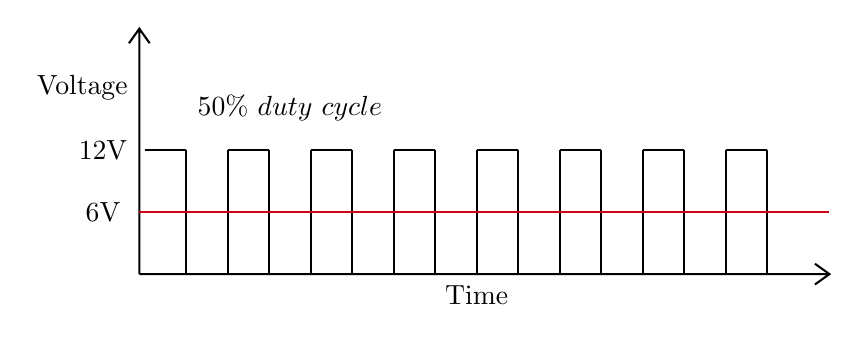
\begin{tikzpicture}[x=0.75pt,y=0.75pt,yscale=-1,xscale=1]
%uncomment if require: \path (0,195.7708282470703); %set diagram left start at 0, and has height of 195.7708282470703

%Shape: Axis 2D [id:dp4590371439594336] 
\draw  (67.5,160) -- (400,160)(67.5,41.77) -- (67.5,160) -- cycle (393,155) -- (400,160) -- (393,165) (62.5,48.77) -- (67.5,41.77) -- (72.5,48.77)  ;
%Straight Lines [id:da2226440769036555] 
\draw    (70,100) -- (90,100) ;


%Straight Lines [id:da027973599787850967] 
\draw    (110,100) -- (130,100) ;


%Straight Lines [id:da43134384380494617] 
\draw    (150,100) -- (170,100) ;


%Straight Lines [id:da4567622353820677] 
\draw    (190,100) -- (210,100) ;


%Straight Lines [id:da06280461715383967] 
\draw    (230,100) -- (250,100) ;


%Straight Lines [id:da7961110488444294] 
\draw    (270,100) -- (290,100) ;


%Straight Lines [id:da2952115332924481] 
\draw    (310,100) -- (330,100) ;


%Straight Lines [id:da347939513568553] 
\draw    (350,100) -- (370,100) ;


%Straight Lines [id:da5371311326985915] 
\draw    (90,100) -- (90,160) ;


%Straight Lines [id:da37558688962973075] 
\draw    (110,100) -- (110,160) ;


%Straight Lines [id:da44168060142753496] 
\draw    (130,100) -- (130,160) ;


%Straight Lines [id:da5162984720027333] 
\draw    (170,100) -- (170,160) ;


%Straight Lines [id:da9328655937237107] 
\draw    (150,100) -- (150,160) ;


%Straight Lines [id:da8698526285458617] 
\draw    (190,100) -- (190,160) ;


%Straight Lines [id:da5579333462058347] 
\draw    (210,100) -- (210,160) ;


%Straight Lines [id:da2831852027876949] 
\draw    (230,100) -- (230,160) ;


%Straight Lines [id:da9724068952844995] 
\draw    (270,100) -- (270,160) ;


%Straight Lines [id:da36611358171538266] 
\draw    (250,100) -- (250,160) ;


%Straight Lines [id:da1948477680776879] 
\draw    (290,100) -- (290,160) ;


%Straight Lines [id:da11576257223436737] 
\draw    (310,100) -- (310,160) ;


%Straight Lines [id:da05602527791808809] 
\draw    (330,100) -- (330,160) ;


%Straight Lines [id:da33311457706338143] 
\draw    (370,100) -- (370,160) ;


%Straight Lines [id:da13026763207224157] 
\draw    (350,100) -- (350,160) ;


%Straight Lines [id:da8029430980655885] 
\draw [color={rgb, 255:red, 208; green, 2; blue, 27 }  ,draw opacity=1 ]   (67.5,130) -- (400,130) ;



% Text Node
\draw (40,70) node  [align=left] {Voltage};
% Text Node
\draw (230,170) node  [align=left] {Time};
% Text Node
\draw (140,80) node   {$50\%\ duty\ cycle$};
% Text Node
\draw (50,100) node  [align=left] {12V};
% Text Node
\draw (50,130) node  [align=left] {6V};


\end{tikzpicture}
    \caption{Illustration of Voltage over time with PWM between 0 and 12V with a duty cycle of 50\%. The read line indicates the average voltage of 6V received by a device}
    \label{fig:PWMUCH}
\end{figure}
\paragraph{Test of "Angle selection."}
The angle select function was tested by inputting, the data from the measuring box into the function.  Through a couple of iteration the setting of AngleChange in \textit{line 4} was changed to find reasonable angle change that made it controllable for the user. 
\subsection*{Visualisation of motor}
\begin{figure}[H]
    \centering
    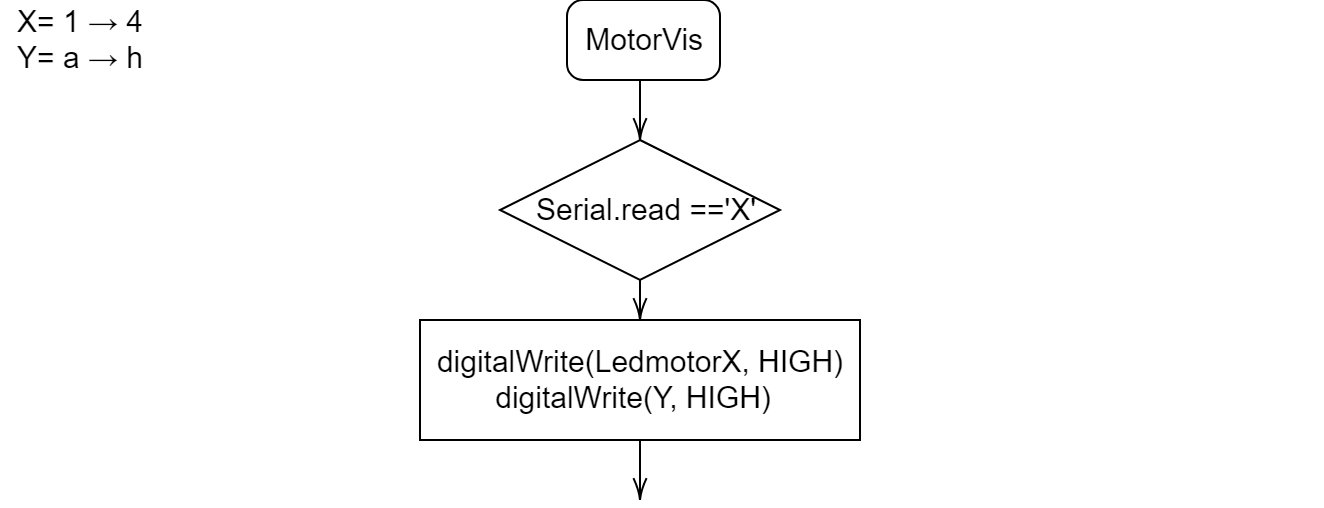
\includegraphics[width=\textwidth]{Figures/Technical_figures/lyskode.png}
    \caption{Flowchart of the MotorVis code}
    \label{fig:motorvis}
\end{figure}
To help the user visualise the motor choice, two methods were used.\\
Firstly two LEDs were placed on each manipulator joint to light up when the joint was chosen, and secondly, a seven segment display was attached to indicate the motor number.
The actual motor number is transmitted from the Teensy as seen in section \ref{MotorSwitchCode} and received by the attached Arduino which runs the code showing the motor choice.

\subsubsection{Code Explanation}

\begin{lstlisting}[frame=single,language=Arduino]
int a = 2;  //For displaying segment "a" on 7 segment sisplay
int b = 3;  //Segment "b"
int c = 4;  //Segment "c"
int d = 5;  //Segment "d"
int e = 6;  //Segment "e"
int f = 7;  //Segment "f"
int g = 8;  //Segment "g"
int h = 9;  //Segment h
int LedMoter1 = 10; // LED on motor one
int LedMoter2 = 11; // LED Moter two
int LedMoter3 = 12; // LED Moter three
int LedMoter4 = 13; // LED Moter four
int incomingByte;      // a variable to read incoming serial data into
void setup() {
  // initialize serial communication:
  Serial.begin(115200);
  // Setup of LEDs and 7seg LED:
  pinMode(a, OUTPUT);
  pinMode(b, OUTPUT);
  pinMode(c, OUTPUT);
  pinMode(d, OUTPUT);
  pinMode(e, OUTPUT);
  pinMode(f, OUTPUT);
  pinMode(g, OUTPUT);
  pinMode(h, OUTPUT);
  pinMode(LedMoter1, OUTPUT);
  pinMode(LedMoter2, OUTPUT);
  pinMode(LedMoter3, OUTPUT);
  pinMode(LedMoter4, OUTPUT);
}
void loop() {
  // see if there's incoming serial data:
  if (Serial.available() > 0) {
    incomingByte = Serial.read();
    if (incomingByte == '1') {
      digitalWrite(LedMoter1, HIGH); delay(1);
      digitalWrite(LedMoter2, LOW); delay(1);
      digitalWrite(LedMoter3, LOW); delay(1);
      digitalWrite(LedMoter4, LOW); delay(1);
      digitalWrite(a, LOW); delay(1);
      digitalWrite(b, HIGH); delay(1);
      digitalWrite(c, HIGH); delay(1);
      digitalWrite(d, LOW); delay(1);
      digitalWrite(e, LOW); delay(1);
      digitalWrite(f, LOW); delay(1);
      digitalWrite(g, LOW); delay(1);
      digitalWrite(h, HIGH); delay(1);
    }
    if (incomingByte == '2') { ...
    }
    if (incomingByte == '3') { ...
    }
    if (incomingByte == '4') { ...
    }
  }
  return;
}
\end{lstlisting} \label{fig:AS}
\begin{figure}[H]
    \centering
    \caption{The source code for visualising of MotorSelect}
\end{figure}




  

\paragraph{Line 1 to 15} The pins are initialised. Integers from \textit{a} to \textit{h} refers to the segments on the seven segment display and the \textit{LedMoter1} to \textit{LedMoter4} is the LEDs attached on each motor. The int \textit{incomingByte} is where the received motor number is written onto.

\paragraph{Line 16 to 35} The \textit{setup} function is used to initialise the variables and define the baudrate. The LED and display segment variables are defined as inputs.

\paragraph{Line 36 to 39} An \textit{if} statement is used to test if the number of characters received from \textit{serial} is grater than zero, as this would indicate data received. \textit{incomingByte} is defined as the motor number value received from serial.

\paragraph{Line 40 to 53} If the received motor number is one, the \textit{if} statement is run and the corresponding LEDs and display segments are turned on/off to show the number one on the display and turn on the LED on motor one. 

\paragraph{Line 55 to 62} The code here are omitted as the structure is identical to the code from line 41 to 53. The segments and LEDs are turned on/off to match the value of \textit{incomingByte} from one to four.

\paragraph{Test of "Visual of representation motor select."}
THe test was initially designed to run on the Teensy 3.5 micro-controller, together with the rest of the code, issues occurred with its implementation. this led to implementing an additional micro controller (arduino uno) in the system, dedicated to running the visualisation code. 
Implementing the code on the arduino, the hardware setup was tested by pre-defining the \textit{incomingByte=2} and commenting out line 33 and 34. The statements were run accordingly, and when confirmed correctly the integer-value were manually changed, to ensure the display and LEDs worked correctly.\\
When the hardware were confirmed to work correctly, line 33 and 34 were implemented and the Arduino were connected to the teensy 3.5 micro controller through the tx and rx pins. The system were turned on, and observed to correctly and reliably show the current joint chosen.


\section{Hardware implementation}
In this section, a description of how the implementation of the hardware is setup is done.
\subsection*{Wire connection}
To have any working parts there is a need to have an understanding of how the different components, that are provided, have to be wired. The wiring of the project was designed upon the different data-sheets and schematics. The first thing to look for is what supply-voltage the different devices can handle, and what pins are used for ground(gnd) and the supply voltage. 
Incorrect supply-voltage and incorrect placement of ground can result in the component not working or even a burnt circuitry.\\
\begin{figure}[H]
    \centering
%\tikzset{every picture/.style={line width=0.75pt}} %set default line width to 0.75pt        

\begin{tikzpicture}[x=0.75pt,y=0.75pt,yscale=-1,xscale=1]
%uncomment if require: \path (0,374); %set diagram left start at 0, and has height of 374

%Image [id:dp7152221511204973] 
\draw (269.48,152.73) node  {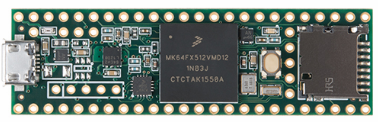
\includegraphics[width=197.45pt,height=60.59pt]{Figures/TikzFigures/layOut/teensy.PNG}};
%Image [id:dp37486105933332636] 
\draw (366.16,279.14) node [rotate=-180.22,xslant=-0.01] {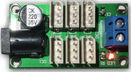
\includegraphics[width=89.36pt,height=69.95pt]{Figures/TikzFigures/layOut/supl.PNG}};
%Image [id:dp9034481830242995] 
\draw (132.79,272.76) node [rotate=-359.65,xslant=0] {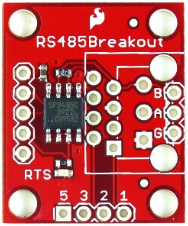
\includegraphics[width=83.35pt,height=72.71pt]{Figures/TikzFigures/layOut/rs.PNG}};
%Image [id:dp11028803786694708] 
\draw (236.5,45.39) node [rotate=-270] {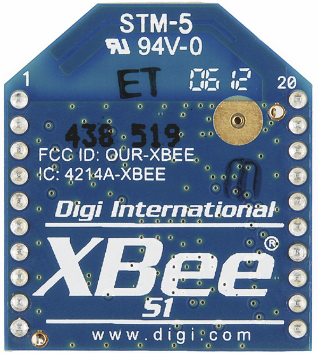
\includegraphics[width=60.59pt,height=62.4pt]{Figures/TikzFigures/layOut/bee.PNG}};
%Left Arrow [id:dp5012443384308891] 
\draw   (438.55,274.06) -- (457.33,256.75) -- (457.33,265.41) -- (485.5,265.41) -- (485.5,282.72) -- (457.33,282.72) -- (457.33,291.38) -- cycle ;
%Right Arrow [id:dp0023557246216043826] 
\draw   (80.2,146.67) -- (111.93,146.67) -- (111.93,137.72) -- (133.09,155.61) -- (111.93,173.5) -- (111.93,164.56) -- (80.2,164.56) -- cycle ;
%Straight Lines [id:da08227247794525927] 
\draw [color={rgb, 255:red, 247; green, 10; blue, 10 }  ,draw opacity=1 ][line width=1.5]    (150.92,81.17) -- (150.52,123.87) ;


%Straight Lines [id:da025924835708441174] 
\draw [color={rgb, 255:red, 247; green, 10; blue, 10 }  ,draw opacity=1 ][line width=1.5]    (217.48,81.17) -- (150.92,81.17) ;


%Straight Lines [id:da00602413999639384] 
\draw [color={rgb, 255:red, 247; green, 10; blue, 10 }  ,draw opacity=1 ][line width=1.5]    (42.76,80.79) -- (155.28,80.79) ;


%Straight Lines [id:da7149252935730617] 
\draw [color={rgb, 255:red, 247; green, 10; blue, 10 }  ,draw opacity=1 ][line width=1.5]    (43.55,80.79) -- (43.55,256.21) ;


%Straight Lines [id:da3829700368795059] 
\draw [color={rgb, 255:red, 247; green, 10; blue, 10 }  ,draw opacity=1 ][line width=1.5]    (91.09,256.21) -- (43.55,256.21) ;


%Straight Lines [id:da8981864779638247] 
\draw [line width=1.5]    (31.67,88.48) -- (31.67,290.84) ;


%Straight Lines [id:da6466608797084847] 
\draw [line width=1.5]    (91.89,290.07) -- (31.67,290.07) ;


%Straight Lines [id:da35185368144106244] 
\draw [line width=1.5]    (31.67,88.48) -- (272.55,89.25) ;


%Straight Lines [id:da8387196090383506] 
\draw    (271.76,80.02) -- (271.76,89.25) ;


%Straight Lines [id:da36845317589148996] 
\draw [color={rgb, 255:red, 91; green, 235; blue, 46 }  ,draw opacity=1 ][line width=1.5]    (225.01,81.56) -- (160.03,184.66) ;


%Straight Lines [id:da4171143722401429] 
\draw [color={rgb, 255:red, 248; green, 231; blue, 28 }  ,draw opacity=1 ][line width=1.5]    (231.55,81.56) -- (173.71,184.66) ;


%Straight Lines [id:da33656991606038633] 
\draw [color={rgb, 255:red, 32; green, 240; blue, 26 }  ,draw opacity=1 ][line width=1.5]    (90.3,273.91) -- (265.42,185.43) ;


%Straight Lines [id:da3740974102672152] 
\draw [color={rgb, 255:red, 244; green, 250; blue, 27 }  ,draw opacity=1 ][line width=1.5]    (255.91,184.66) -- (91.89,265.45) ;


%Straight Lines [id:da18281067478913027] 
\draw [color={rgb, 255:red, 74; green, 144; blue, 226 }  ,draw opacity=1 ][line width=1.5]    (91.09,282.37) -- (276.51,185.43) ;


%Straight Lines [id:da7137403407481466] 
\draw [line width=1.5]    (180.34,279.84) -- (343.47,319.08) ;


%Straight Lines [id:da9319303523938192] 
\draw [color={rgb, 255:red, 243; green, 20; blue, 20 }  ,draw opacity=1 ][line width=1.5]    (180.34,271.18) -- (344.5,305) ;


%Straight Lines [id:da7229658725423573] 
\draw [color={rgb, 255:red, 74; green, 144; blue, 226 }  ,draw opacity=1 ][line width=1.5]    (180.34,262.52) -- (343.5,296) ;


%Straight Lines [id:da43545523008986176] 
\draw [line width=1.5]    (31.5,202) -- (150.5,202) ;


%Straight Lines [id:da5107595655280059] 
\draw [line width=1.5]    (150.5,183) -- (150.5,202) ;



% Text Node
\draw (99.41,156.19) node  [align=left] {USB};
% Text Node
\draw (465.49,273.68) node  [align=left] {12V};
% Text Node
\draw (77,191) node  [align=left] {Gnd};
% Text Node
\draw (98,71) node  [align=left] {5V};
% Text Node
\draw (257,310) node  [align=left] {Gnd};
% Text Node
\draw (263,265) node  [align=left] {Rs 485};
% Text Node
\draw (338,106) node  [align=left] {Teensy 3.5};
% Text Node
\draw (133,341) node  [align=left] { \ \ \ BOB-10124\\Rs 232 to Rs 485};

% Text Node
\draw (212,108) node  [align=left] {Rx1 \ \ \ Tx1};
% Text Node
\draw (192,199) node  [align=left] {RxTx2};
% Text Node
\draw (317,212) node  [align=left] {Transmit enable wire};


\end{tikzpicture}
    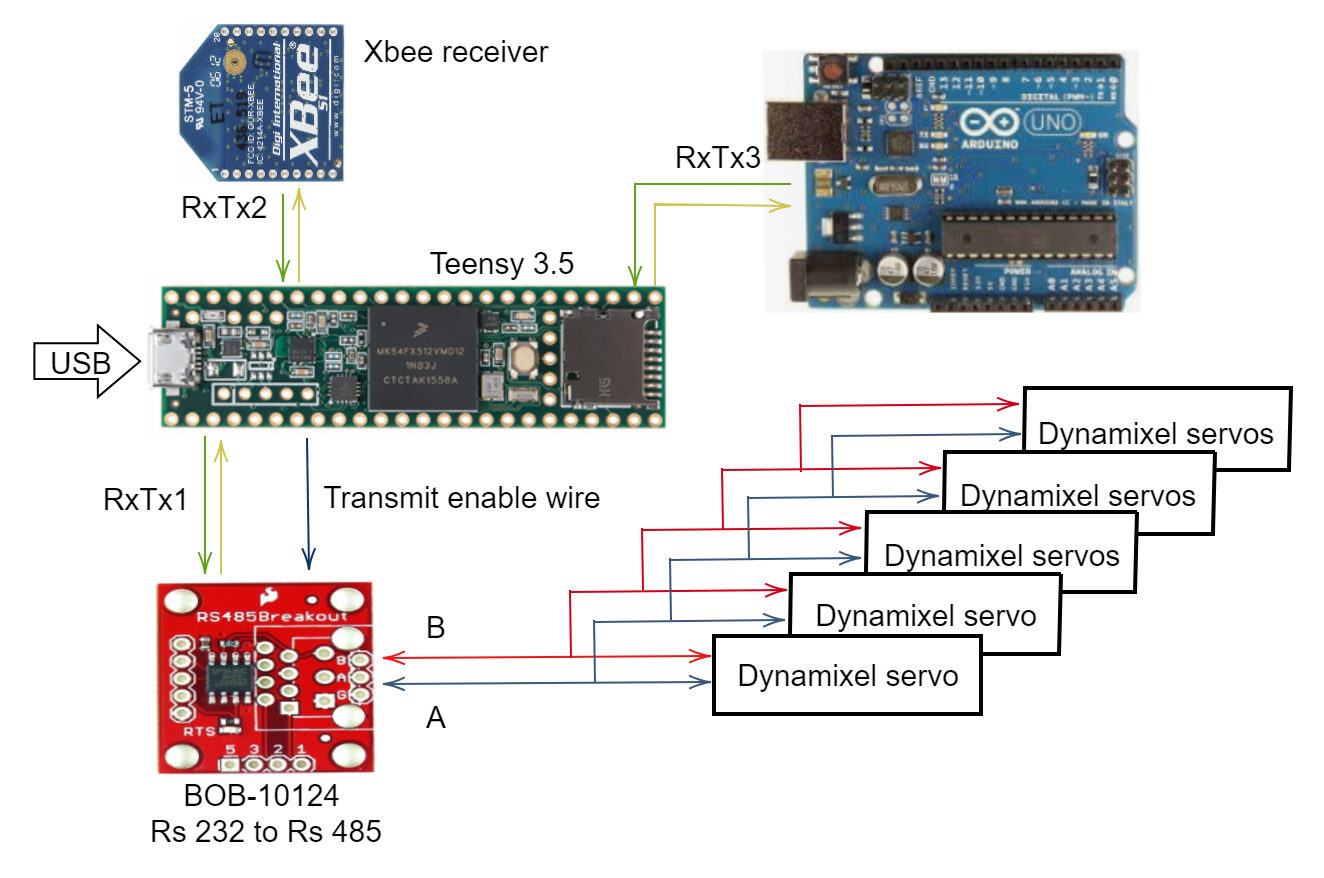
\includegraphics[scale=0.30]{Figures/Technical_figures/HWlayout.png}
    \caption{Wiring of the Teensy to external components}
    \label{fig:motorSel}
\end{figure}
The next thing to look for is which communication protocol the different components utilises. This is important because different protocols do not work together. All this can be found on the data sheets provided by the manufacturers of each components.
\paragraph{Test of "Connection between devices."}
The of correct wiring was first carried out trough a visual inspection of the wiring before applying any power to the system. After visual inspection the power supply was turn on, luckily there was no "Magic smoke" appearing. That meant it was possible to check for connectivity between Teensy, CrustCrawler, measuring box and the Arduino that controllers the light on the CrustCrawler.
By only adding one new component to the Teensy a time, it was easier to control the debugging of the connection between each component.

\subsection*{Visualisation of motor}
For the user to have a clear overview of which servo is in use, a 7 segment display is used to display what number of motor, the user has selected within the function \textbf{MotorSwitch}.
\begin{figure}[H]\label{SchematicOfLED}
    \centering
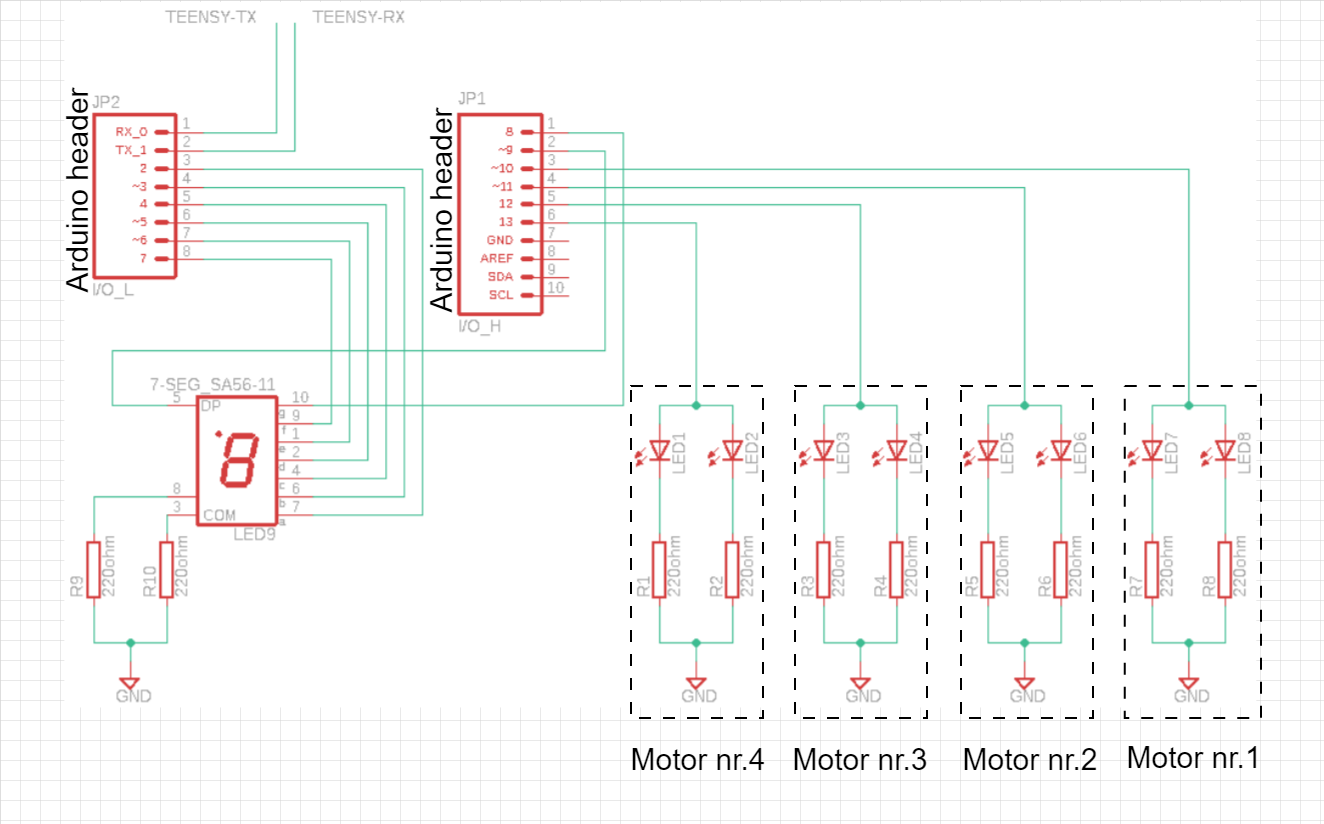
\includegraphics[width=\textwidth]{Figures/Technical_figures/hwLEd.png}
    \caption{Schematic of visual motor representation}
    \label{fig:VismotorSel}
\end{figure}
 Furthermore 2 LED's was placed on each motor, each pair of LED's will illuminate when the particular motor is selected. The control of these LED's is done through another microcontroller(Arduino Uno), that is connected through RS-232 serial communication. This configuration allows the Teensy to have more time to process the data inputs from the measuring box, and focus on the control of the motors.
 \paragraph{Test of "Hardware implementation of visual representation."}
 This test was done through visual inspection. By looking at the selected motor in the GUI and looking at what LED that was illuminated and what number was displayed in the 7-segment display.
 The test was a success and will aid the user in a more precises control of the CrustCrawler by visual cue's.
 
 